\section{Lengthy Pregnancy}
If offspring are produced immediately upon consumption, then the setup where starvation is the only way to die
leads to immediate consumption of all resources being the optimal strategy. Here we alter the setup of squirrel
banking slightly so that pregnancy lasts a full time step rather than being an immediate translation into offspring.
For the demographic structure, this means that we have a category for each savings level $\beta\in\left\{ 0
, 1, \ldots, \hat \beta\right\}$, as well as an additional ``pregnant'' category. There are two natural families
of Leslie/population matrices which encompass all of this information. The first family of matrices assumes that,
while pregnant, a squirrel cannot get pregnant again. If a second nut is found, it is incapable of doing anything
different than if it had found one nut.

$$L_0 = 
\begin{bmatrix}
    p_1 & 2(p_1 + p_2) \\
    p_2 & 0
\end{bmatrix}
$$

$$ L_1 =
\begin{bmatrix}
    p_1 & p_0 & 1 + p_0 \\
    p_2 & p_1 & p_1 + p_2 \\
    0 & p_2 & 0
\end{bmatrix}
$$
$$L_{\hat \beta} = 
\begin{bmatrix}
    p_1 & p_0 & 0 & \cdots & 0 & 1 \\
    p_2 & p_1 & p_0 & \cdots & 0 & 0 \\
    0 & p_2 & p_1 & \cdots & 0 & 0 \\
    \vdots & \vdots & \vdots & \ddots & \vdots & \vdots \\
    0 & 0 & 0 & \cdots & p_0 & p_0 \\
    0 & 0 & 0 & \cdots & p_1 & p_1 + p_2 \\
    0 & 0 & 0 & \cdots & p_2 & 0 \\
\end{bmatrix}
$$

The second family of matrices assumes that if a second nut is found while pregnant, the squirrel preemptively gets pregnant
for the second day in a row. 

$$L_0 = 
\begin{bmatrix}
    p_1 & 2p_1 + p_2 \\
    p_2 & p_2
\end{bmatrix}
$$

$$ L_1 =
\begin{bmatrix}
    p_1 & p_0 & 1 + p_0 \\
    p_2 & p_1 & p_1 \\
    0 & p_2 & p_2 
\end{bmatrix}
$$
$$L_{\hat \beta} = 
\begin{bmatrix}
    p_1 & p_0 & 0 & \cdots & 0 & 1 \\
    p_2 & p_1 & p_0 & \cdots & 0 & 0 \\
    0 & p_2 & p_1 & \cdots & 0 & 1 \\
    \vdots & \vdots & \vdots & \ddots & \vdots & \vdots \\
    0 & 0 & 0 & \cdots & 0 & p_0 \\
    0 & 0 & 0 & \cdots & p_1 & p_1  \\
    0 & 0 & 0 & \cdots & 0 & p_2 \\
\end{bmatrix}
$$

In the present context, it is natural to wonder: what is the optimal $\hat \beta$ given a triple $(p_0, p_1, p_2)$? Does the imposition of a 
day long pregnancy which must be survived incentivize to save a stock of nuts before beginning procreation? The answer is yes. Empirically,
I find that squirrels are always better off by saving at least to $\hat \beta = 1$ before producing offspring; whether $\hat \beta > 1$ depends
on where in the simplex $\left\{ \left( p_0, p_1, p_2 \right): \sum p_i = 1 \right\}$ the squirrel finds itself. For the first family of squirrels,
the results are summarized in the following ternary plots:

\begin{figure}[H]
    \centering
    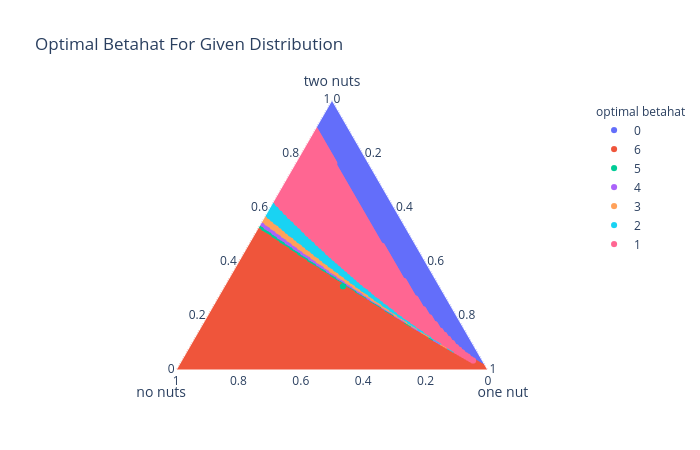
\includegraphics[scale = 0.8]{optimal_betahat_Aug17} \\
\end{figure}
\begin{figure}[H]
    \centering
    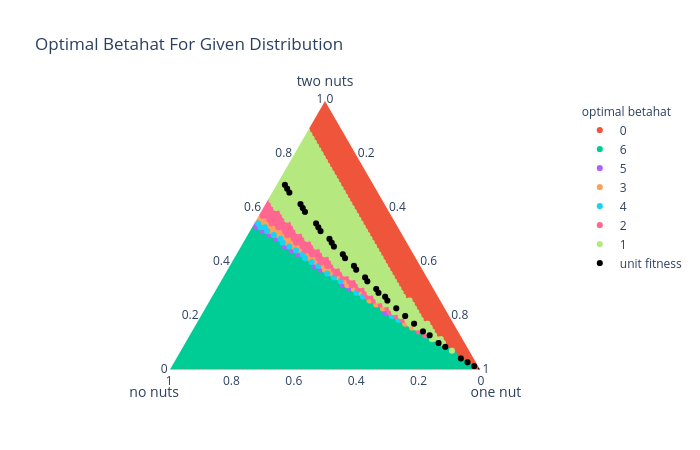
\includegraphics[scale = 0.8]{overlaid_unit_fitness} \\
\end{figure}
\begin{figure}[H]
    \centering
    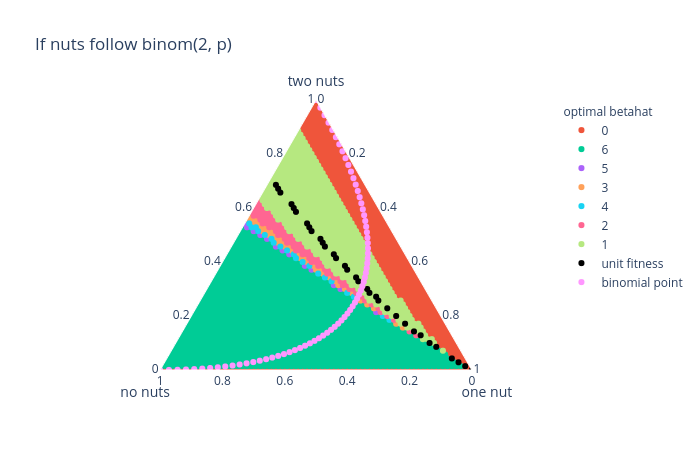
\includegraphics[scale = 0.8]{overlaid_binom} \\
\end{figure}
\begin{figure}[H]
    \centering
    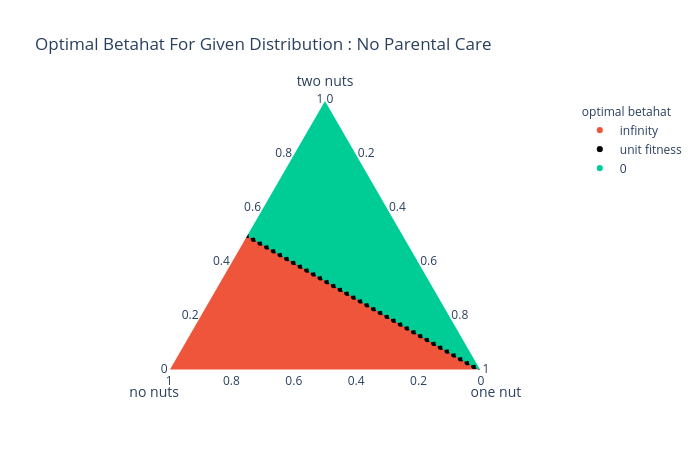
\includegraphics[scale = 0.8]{unit_fitness_no_pc} \\
\end{figure}


Courtesy of Jaye's suggestion, I'll start using the terminology Parental Care for what has until now been called ``pregnancy.'' 
The idea right now is to get some intuition for why squirrels make the decisions they do. Of course, we have computed the different
fitnesses and thus the optimal $\hat \beta$ is indisputable, but the indifference arcs (for example, between $\hat \beta = 0, 1$) seem
to be drawn arbitrarily. Why are those arcs where they are? And can we get some intuition for why exactly we need ever increasing
values of $\hat \beta$ to fill the entire half of the simplex with $p_2 > p_0$?  \\ \\
Fitness can be thought of as defined by
$$ r = 1 + b - d $$
where $b,d$ are respectively the birth and death rates of the population. Take as given a demographic matrix $L$, its leading eigenvalue
$r$, and its corresponding eigenvector $\left( n_0, n_1, \ldots, n_{\hat \beta}, n_{PC} \right)$ normalized
such that $\sum n_k = 1$. In a given time step, we can expect that anybody surviving the period of parental care gives birth; at the same time,
any squirrel with zero nuts banked and who finds zero nuts will die. This gives
\begin{itemize}
    \item $b = n_{PC}$ or $b = (1 - p_0)n_{PC}$ if $\hat \beta = 0$,
    \item $d = n_0p_0$.
\end{itemize}
In sum,

$$ r_{\hat \beta} =
\begin{cases}
    1 + n_{PC}^{\hat \beta}\left( 1 - p_0 \right) - n_0^{\hat \beta}p_0 & \text{ if  } \hat \beta = 0 \\
    1 + n_{PC}^{\hat \beta} - n_0^{\hat \beta}p_0 & \text{ if  } \hat \beta \ge  1
\end{cases}
$$

%Notice $n_{PC} = p_2 n_{\hat \beta}$, so
%$$ r_{\hat \beta} =
%\begin{cases}
%    1 + p_2n_{\hat \beta}^{\hat \beta}\left( 1 - p_0 \right) - n_0^{\hat \beta}p_0 & \text{ if  } \hat \beta = 0 \\
%    1 + p_2n_{\hat \beta}^{\hat \beta} - n_0^{\hat \beta}p_0 & \text{ if  } \hat \beta \ge  1
%\end{cases}
%$$
Intuitively, increasing $\hat \beta$ decreases the value of each $n_k$. The intuition is that increasing the number
of bins decreases how much we can put in each bin. 
%For each increase in $\hat \beta$, we (experimentally) find
%that $n_{PC}$ decreases by about half as much as $n_0$. 
To gain an intuitive appreciation for the positioning of the indifference
arcs, consider the following. Assume $\hat \beta \ge 1$ (so we don't have to deal with the $\hat \beta = 0$ case from above). Then:

\begin{align*}
    r^{\hat \beta} \le r^{\hat \beta + 1} &\iff  n_{PC} - p_0n_0 \le n_{PC}' - p_0n_0' \\
    &\iff n_{PC} - n_{PC}' \le p_0\left( n_0 - n_0' \right) \\
    &\iff \frac{n_{PC} - n_{PC}'}{n_0 - n_0'} \le p_0
\end{align*}

The above is a bit notationally dense. We use primes to denote the leading eigenvector of $L_{\hat \beta + 1}$; that is,
$n$ is such that $L_{\hat \beta} n = r^{\hat \beta}n$ and $n'$ is such that $L_{\hat \beta + 1}n' = r^{\hat \beta + 1}n'$. 
We therefore have a condition for choosing to save to $\hat \beta + 1$, given our position in the simplex: compute 
$$ f\left( p_0, p_1, \hat \beta \right) := \frac{ \Delta n_{PC}}{\Delta n_{0}} $$
and compare with the constant $p_0$.  \\ \\

Another tangent. It is clear upon reflection that $n_{PC} = \frac{p_2 n_{\hat \beta}}{r_{\hat \beta}}$. Then 
\begin{align*}
    r &= 1 + n_{PC} - p_0n_0 \\
    r &= 1 + \frac{p_2 n_{\hat \beta}}{r} - p_0 n_0 \\
    r^2 &= (1 - p_0n_0)r + p_2n_{\hat \beta} \\
    0 &= r^2 + \left( p_0n_0 -1 \right)r - p_2n_{\hat \beta},
\end{align*}
to which we can apply the quadratic formula to obtain
$$ r = \frac{ 1 - p_0n_0 \pm \sqrt{\left( 1 - p_0n_0 \right)^2 + 4p_2n_{\hat \beta}}}{2}. $$
Since $n_k\to0$ for each $k$ as $\hat \beta\to \infty$, we can conclude that 
$r\to0, 1$ as $\hat \beta\to \infty$. This, after some thought, is intuitive; if an infinitely large population of squirrels
somehow managed to get to stable savings distribution, then almost nobody dies and almost nobody reproduces, so that the population remains
stable irrespective of the distibution of nuts.  \\\\

We can leverage the quadratic formula expression above to get a nice result. We have $r_{\hat \beta} > 1$ iff
\begin{align*}
    \frac{ 1 - p_0n_0 + \sqrt{(1 - p_0n_0)^2 + 4p_2n_{\hat \beta}}}{2} &\ge 1 \\
    \sqrt{(1 - p_0n_0)^2 + 4p_2n_{\hat \beta}} &\ge 1 + p_0n_0 \\
    (1 - p_0n_0)^2 + 4p_2n_{\hat \beta}  &\ge \left( 1 + p_0n_0 \right)^2 \\
    4p_2n_{\hat\beta} &\ge 4p_0n_0 \\
    p_2n_{\hat\beta} &\ge p_0n_0
\end{align*}

The above expression agrees with my historic intuition. I \textit{wanted} to say that $n_{PC} = p_2n_{\hat \beta}$, but that,
it turns out, is false. But we get the exact same condition for $r_{\hat \beta} > 1$ as if it did hold. Cool!

